\documentclass[11pt, a4paper]{article}
\usepackage[utf8]{inputenc}
\usepackage{geometry}
\usepackage{graphicx}
\usepackage{float}
\usepackage{amsmath}
\usepackage[dvipsnames]{xcolor}
\geometry{margin=1in}
\setlength{\parindent}{0em}
\setlength{\parskip}{1em}
\title{Computação Gráfica | Trabalho 3}
\author{Professor: Waldemar Celes\\
Aluno: Antenor Barros Leal}
\date{01 de dezembro de 2024}
\begin{document}
\maketitle

\section {Resumo}
Este trabalho tem como objetivo fazer a implementação e teste de técnicas de renderização
em uma cena 3D.

\section {Cena Base}
Para a cena utilizou-se uma versão com leves modificações a partir da tarefa 2.1. 

Para este trabalho o cubo cinza foi retirado para ser substituído por um quad 
que fará papel de uma superfície plana para o refletor e como anteparo para a 
projeção das sombras.

O seguinte grafo de cena foi usado:

\begin{verbatim}
  Node::Make(shader,
      {
          Node::Make(trCube2,{yellow},{cube}),
          Node::Make(trSphere1,{green},{sphere}),
          Node::Make(trSphere2,{red},{sphere}),
          Node::Make(trCube3,{red},{cube}),
      }
  );
\end{verbatim}

\section {Técnicas de Renderização}

Entre as opções, foi escolhido a técnica de reflexão planar e de sombra planar.

\subsection {Técnica: reflexão planar}

Como dito na seção anterior foi usado um quad para receber a reflexão que é 
simplesmente a repetição da cena em $$y > 0$$ em $$y < 0$$ com a componente y
com sinal trocado. Usando o transformador de escala conseguimos fazer esta 
inversão:

\begin{verbatim}
trf->Scale(1.0f,-1.0f,1.0f);
\end{verbatim}

Todavia, se apenas isto for feito, a reflexão irá "vazar" para fora da superficie
reflexiva.

\begin{figure}[H]
  \begin{center}
  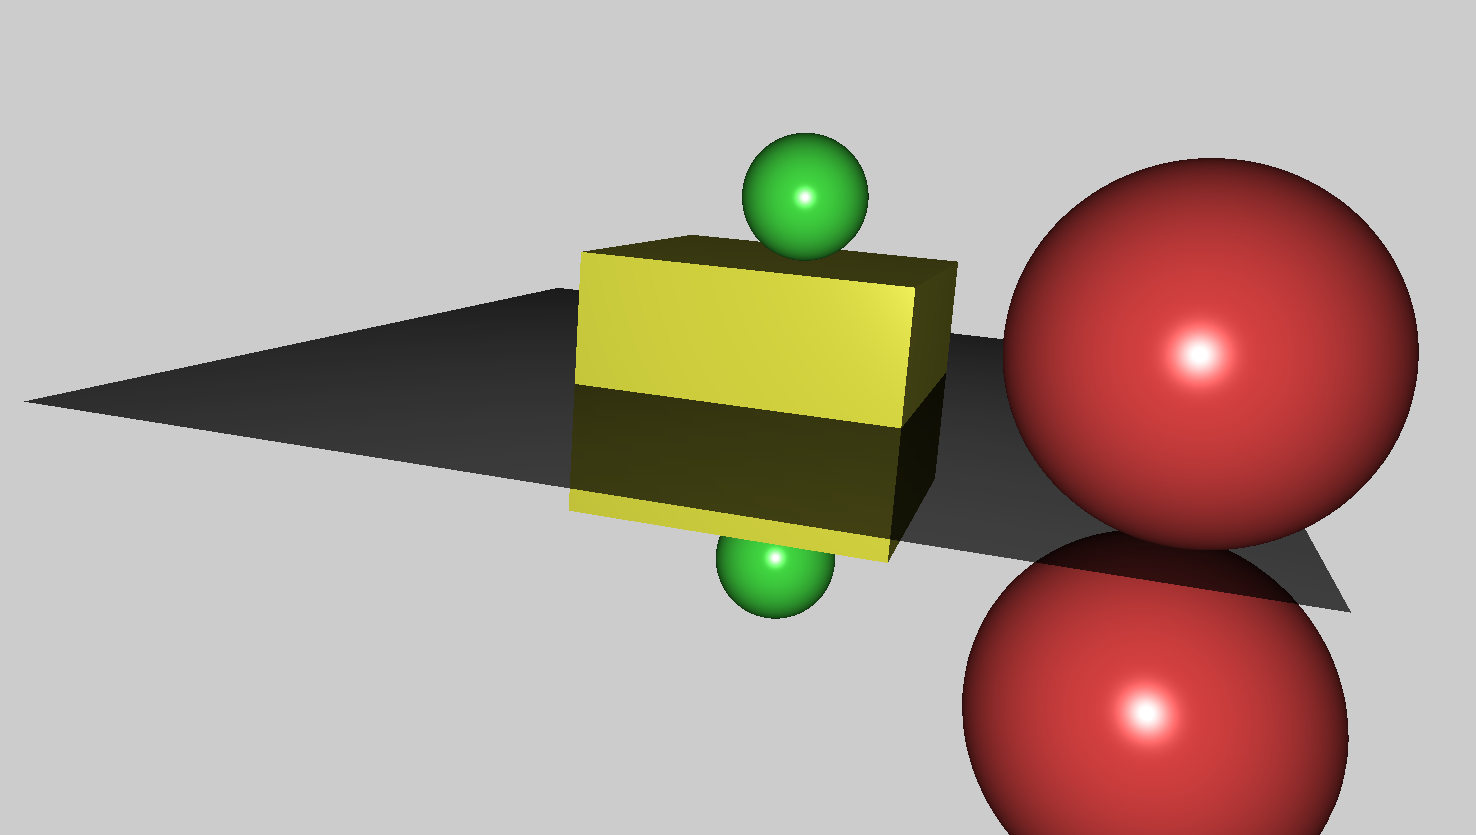
\includegraphics[width=0.8\linewidth]{before-stencil.png}
  \caption{Antes do stencil}
  \label{fig:vaz}
  \end{center}
\end{figure}

Isto é resolvido aplicado um stencil na superficie reflexiva e informado ao 
ao OpenGL não renderizar a reflexão que esteja fora desta máscara.

\begin{figure}[H]
  \begin{center}
  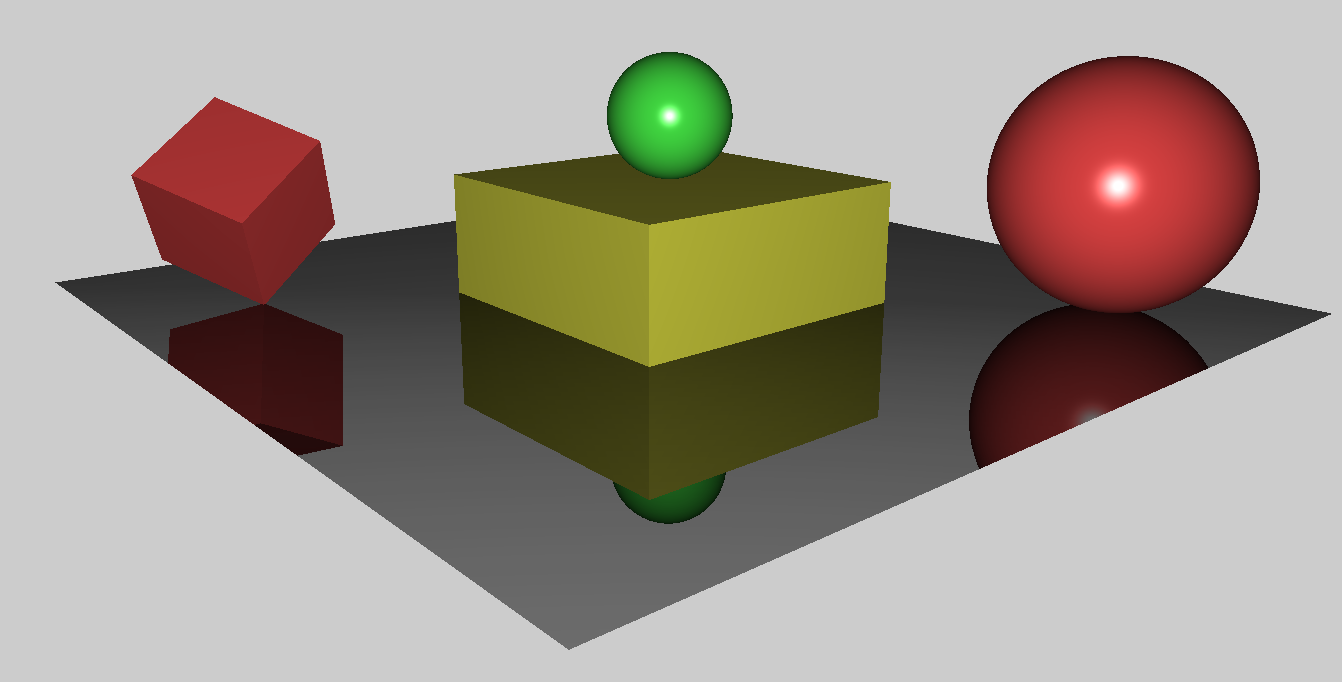
\includegraphics[width=0.8\linewidth]{after-stencil.png}
  \caption{Depois do stencil}
  \label{fig:vaz}
  \end{center}
\end{figure}

Porém se mudarmos o arcball para visualizar a parte de baixo da superficie reflexiva, 
vemos parte do reflexo cortado pelo stencil. O que se é desejado, obviamente, é 
a ausência de qualquer objeto.

\begin{figure}[H]
  \begin{center}
  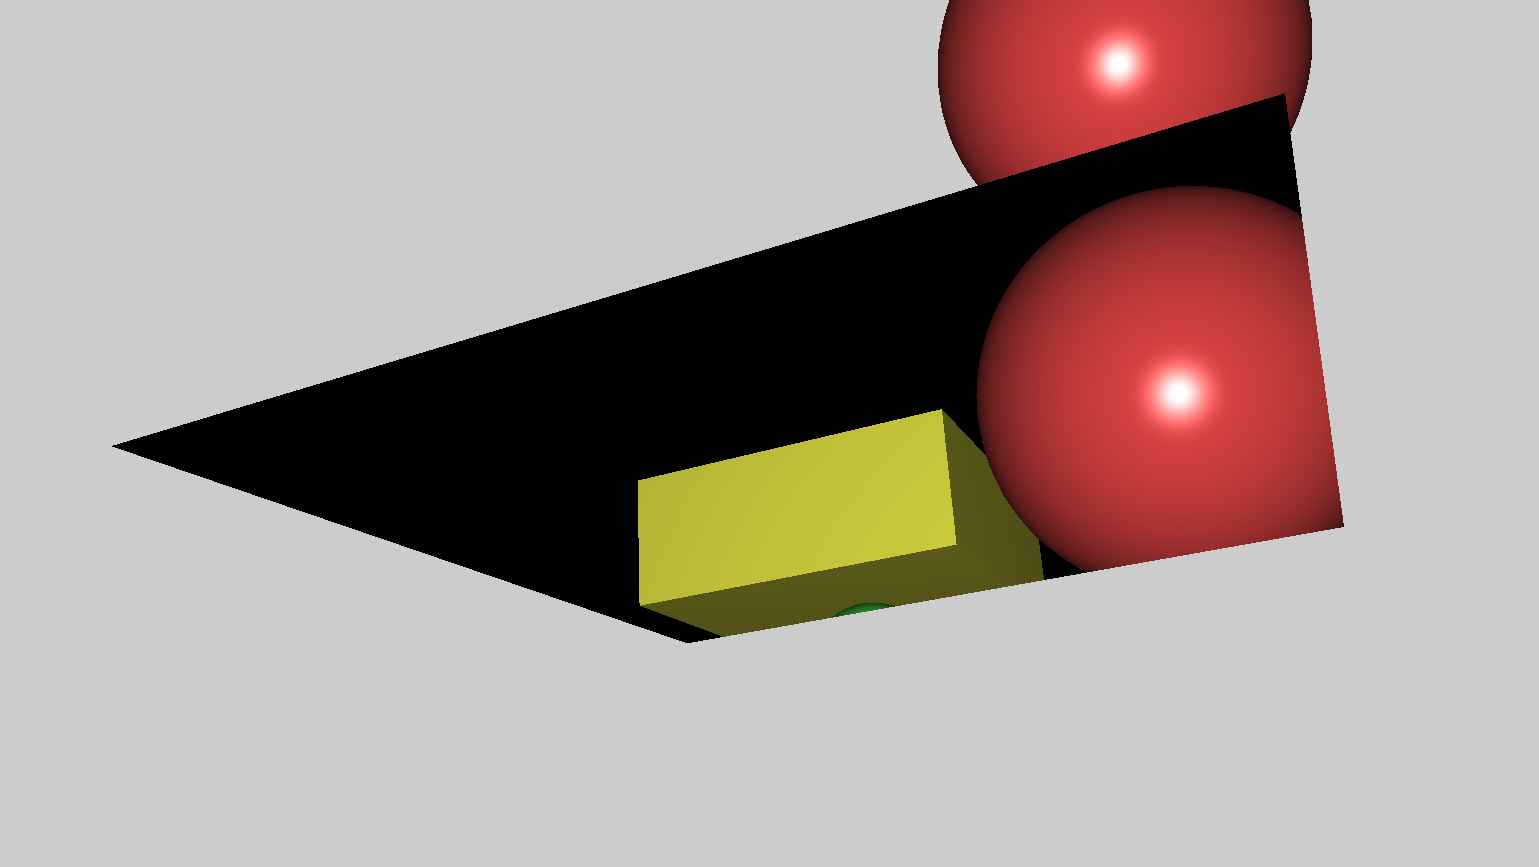
\includegraphics[width=0.8\linewidth]{before-cut-plan.png}
  \caption{Antes do plano de corte}
  \label{fig:vaz}
  \end{center}
\end{figure}

Para resolver isso usamos um plano de corte para mostrar a cena refletida apenas
acima do plano de corte.


\subsection {Técnica: sombra planar}

Para a sobra planar aplicamos a geometria em uma matriz de projeção que "achata"
os objetos de cena em uma superficie 2D. Esta matriz de projeção por considerar a posição da luz
consegue simular corretamente como é a sombra projetada por esta luz.

\subsection{Matriz de projeção}

Sendo n o vetor de quatro índices (1x4) represetando a normal ao plano onde a sombra deve
ser exibida com os três primeiros índices igual as componentes x, y e z e o último
índice sendo fixo igual à um.

Sendo, l o vetor também de quatro índices com a posição x, y, z da fonte de luz 
e o quarto índice também igual à um.

Os pontos de geometria, quando forem multiplicados pela matriz:

\[
\begin{bmatrix}
  nl + n_{w} - l_{x}n_{x} & -l_{x}n_{y} & -l_{x}n_{z} & -l_{x}n_{w} \\
  -l_{y}n_{x} & nl + n_{w} - l_{y}n_{y} & -l_{y}n_{z} & -l_{y}n_{w} \\
  -l_{z}n_{x} & -l_{z}n_{y} & nl + n_{w} - l_{z}n_{z} & -l_{z}n_{w} \\
  -n_{x} & -n_{y} & -n_{z} & nl
\end{bmatrix}
\]

Serão transformados em pontos que formam a sombra planar.

\subsection{Algorítmo}
Para renderizar a cena, faz-se quatro passadas. Inicialmente é limpado o stencil 
porque se não teríamos um efeito de "pintura" já que as marcações do stencil 
iriam se acumular de quadro a quadro.

\begin{verbatim}
glClear(GL_COLOR_BUFFER_BIT | GL_DEPTH_BUFFER_BIT | GL_STENCIL_BUFFER_BIT);
\end{verbatim}

Modifiquei o shader para que fosse possível renderizar a cena apenas com a luz 
ambiente caso uma variável fosse verdadeira.

\begin{verbatim}
if (amb_only) {
  fcolor = ambient;
}
else {
  fcolor = ambient + diffuse + specular;
}
\end{verbatim}

Na primeira passada é renderizado o chão apenas com a luz ambiente.

\begin{verbatim}
amb_only->SetValue(true);
sceneGround->Render(camera);
amb_only->SetValue(false);
\end{verbatim}


Na segunda passada a geometria da cena é multiplicada pela matriz de sombra e o 
stencil é marcado com a resultante. Esta marcação é a sombra.

\begin{verbatim}
glEnable(GL_STENCIL_TEST);
glStencilFunc(GL_NEVER , 1, 0xFFFF);
glStencilOp(GL_REPLACE , GL_REPLACE , GL_REPLACE);
glm::mat4 sm = shadowMatrix(glm::vec4(0.0f,0.0f,1.0f,1.0f),glm::vec4(2.0f, 2.0f, 
10.0f, 1.0f));
TransformPtr tr = Transform::Make();
//tr->LoadIdentity();
tr->MultMatrix(sm);
sceneRoot->GetRoot()->SetTransform(tr);
sceneRoot->Render(camera);
sceneRoot->GetRoot()->SetTransform(nullptr);
\end{verbatim}

Na terceira passada o chão é desenhado normalmente, exceto pelas áreas onde o 
stencil foi marcado. Nestas áreas apenas a luz ambiente do passo anterior irá 
aparecer.

\begin{verbatim}
glStencilFunc(GL_EQUAL , 0, 0xFFFF);
glStencilOp(GL_KEEP , GL_KEEP , GL_KEEP);
glBlendFunc(GL_ONE ,GL_ONE);
glEnable(GL_BLEND);
glDepthFunc(GL_EQUAL);
sceneGround->Render(camera);
glDepthFunc(GL_LESS);
glDisable(GL_STENCIL_TEST);
glDisable(GL_BLEND);
\end{verbatim}

Por fim, a cena principal é desenhada normalmente.

\begin{verbatim}
sceneRoot->Render(camera);
\end{verbatim}

\begin{figure}[H]
  \begin{center}
  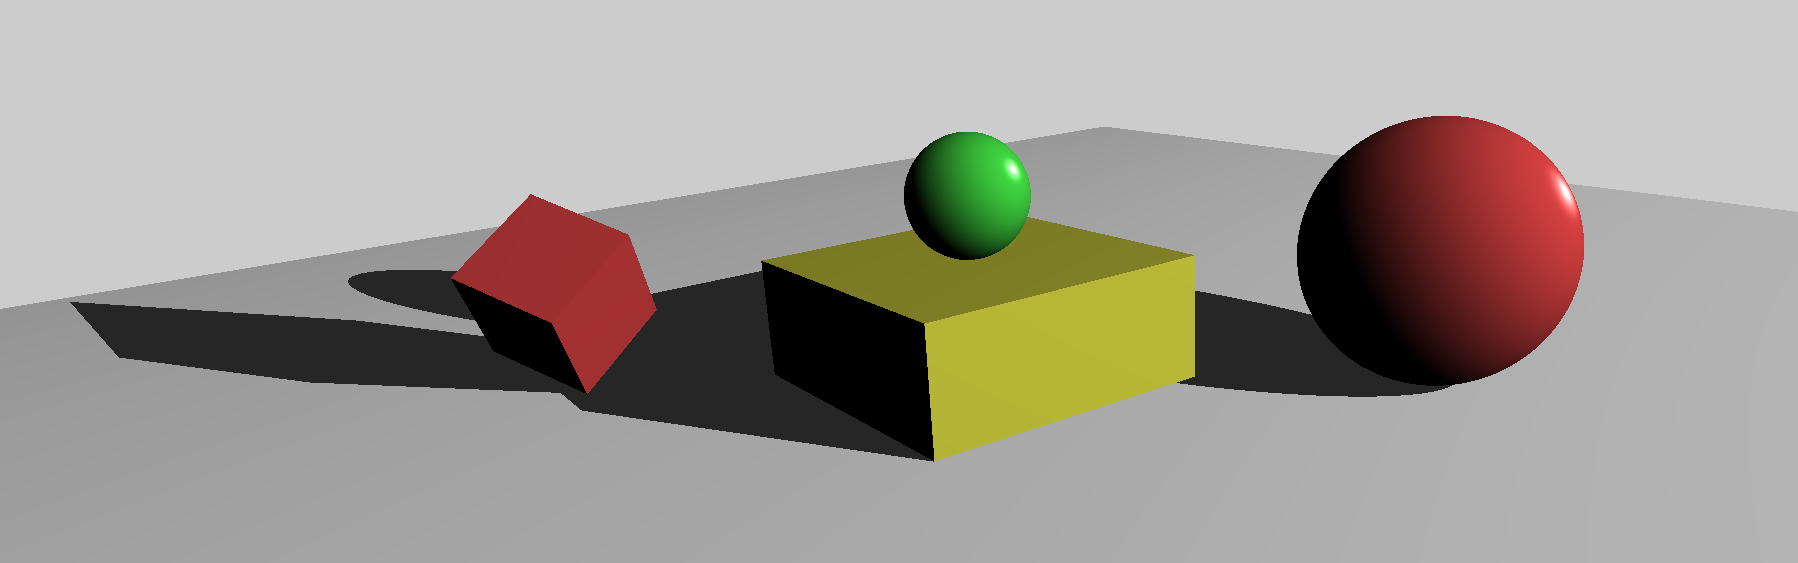
\includegraphics[width=0.8\linewidth]{shadow.png}
  \caption{Cena com sombra}
  \label{fig:vaz}
  \end{center}
\end{figure}

\begin{figure}[H]
  \begin{center}
  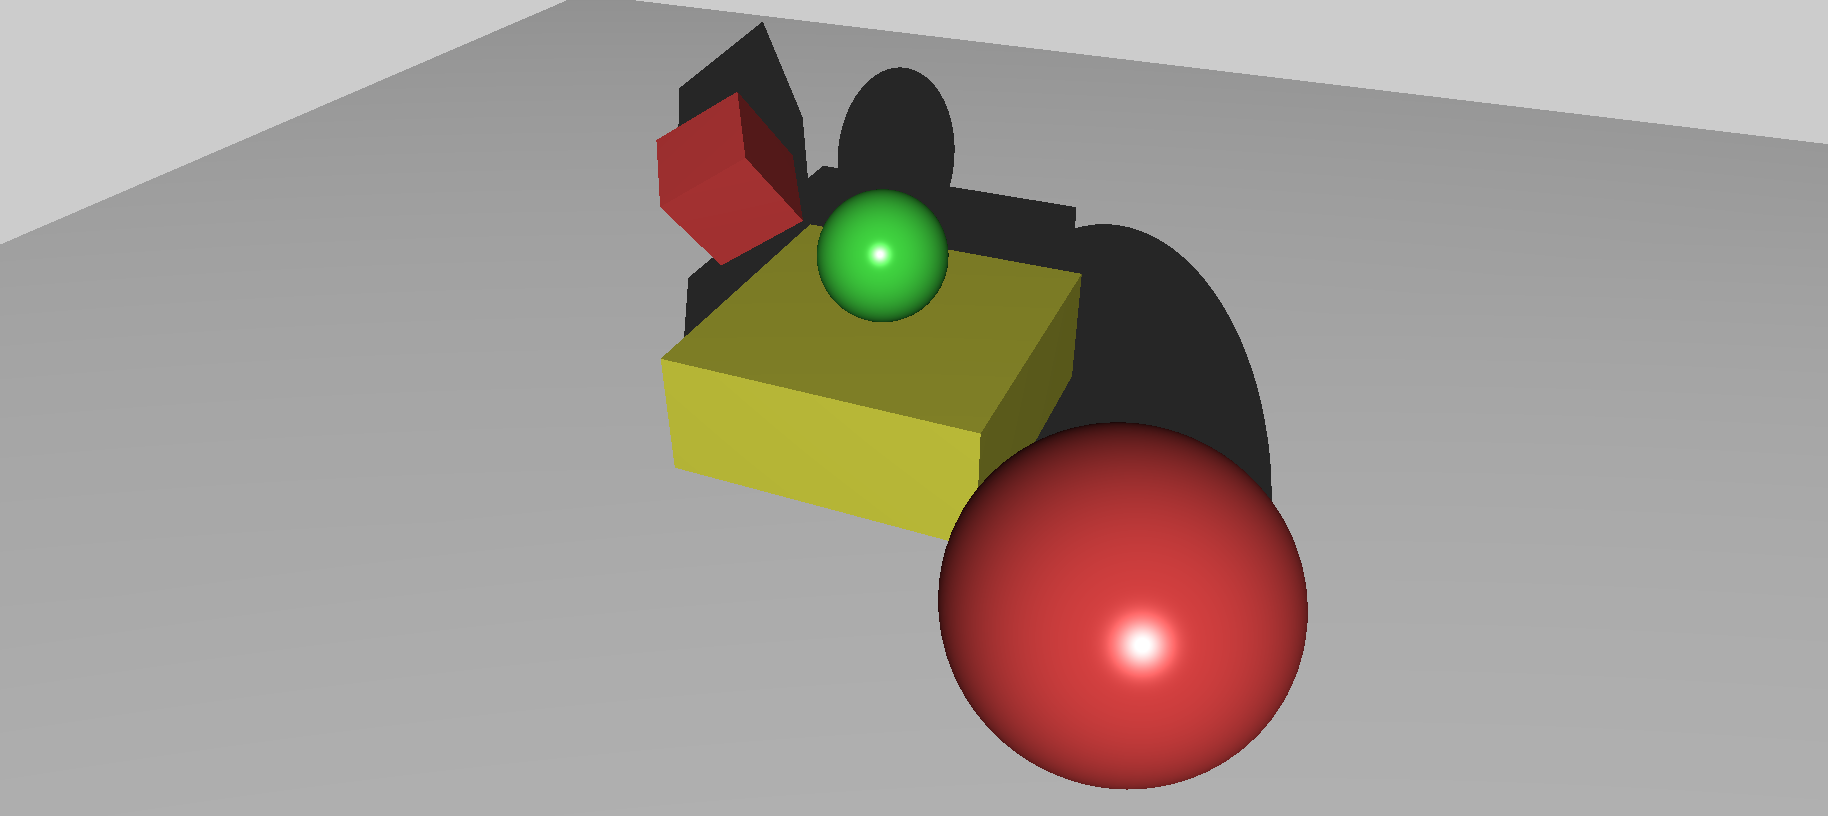
\includegraphics[width=0.8\linewidth]{shadow-2.png}
  \caption{Cena com sombra 2}
  \label{fig:vaz}
  \end{center}
\end{figure}

\section {Resultados}

Além das capturas de tela deste relatório, um vídeo de demostração do funcionamento 
foi incluído: arquivo "demo.mp4".

\end{document}